% diagrams/english/rosco.tex -- el King cake, el roscón de Reyes, para
% "Read and colour": el rosco (redondo como un anillo), las frutas de
% encima, la guinda y la corona de papel en el agujero de en medio.
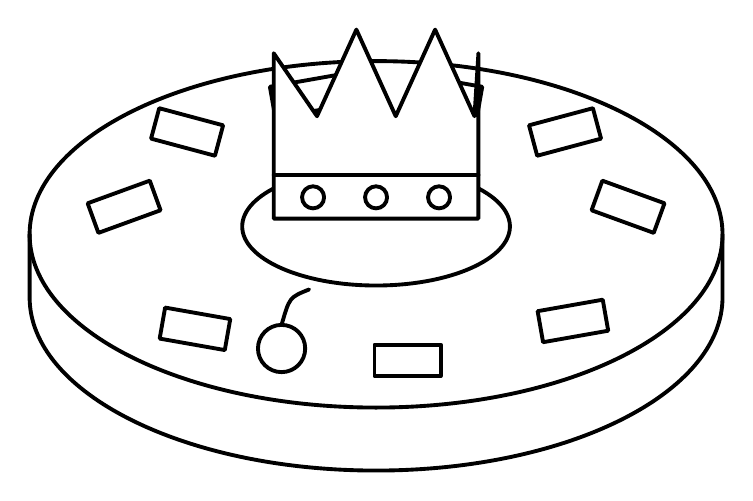
\begin{tikzpicture}[line width=1.4pt, line cap=round, line join=round, scale=1.0]
  % el rosco: dos elipses, y el borde de delante
  \filldraw[fill=white] (0,0) ellipse (4.4 and 2.2);
  \draw (-4.4,0) -- (-4.4,-0.8) arc (180:360:4.4 and 2.2) -- (4.4,0);
  \filldraw[fill=white] (0,0.1) ellipse (1.7 and 0.75);
  % las frutas de encima, cada una cerrada
  \foreach \x/\y/\g in {-3.2/0.35/20, -2.4/1.3/-15, -0.9/1.75/10, 0.9/1.75/-10,
                        2.4/1.3/15, 3.2/0.35/-20, 2.5/-1.1/10, 0.4/-1.6/0, -2.3/-1.2/-10} {
    \begin{scope}[shift={(\x,\y)}, rotate=\g]
      \filldraw[fill=white] (-0.42,-0.2) rectangle (0.42,0.2);
    \end{scope}
  }
  % la guinda
  \filldraw[fill=white] (-1.2,-1.45) circle (0.3);
  \draw (-1.2,-1.15) .. controls (-1.1,-0.8) .. (-0.85,-0.7);
  % la corona de papel, de pie en el agujero
  \filldraw[fill=white] (-1.3,0.2) -- (-1.3,2.3) -- (-0.75,1.5) -- (-0.25,2.6) -- (0.25,1.5)
    -- (0.75,2.6) -- (1.25,1.5) -- (1.3,2.3) -- (1.3,0.2) -- cycle;
  \draw (-1.3,0.75) -- (1.3,0.75);
  \foreach \x in {-0.8,0,0.8} { \filldraw[fill=white] (\x,0.47) circle (0.14); }
\end{tikzpicture}
